\documentclass[10pt,letter]{article}
\usepackage{amsmath,amssymb,graphicx,setspace,fullpage,breqn}
\onehalfspacing
\usepackage{fullpage}

\begin{document}
\paragraph*{I.} \textbf{Bijection between order ideals in $\lambda \times [n]$ and increasing tableaux.} This generalizes Theorem 4.1 to posets whose base shape is any connected subset of $\mathbb{Z}^{d-1}$. 

\subparagraph*{Background.}

We call a nonempty finite subset $\lambda \subset \mathbb{Z}^{d-1}$ a \textit{shape}. Let $e_i$ be the standard basis vector in $\mathbb{R}^{d-1}$. Let $\pi_1(x)$ be the projection onto the $i^{th}$ coordinate.

We say that $\lambda$ is \textit{convex} if whenever $x$ and $x + k \, e_i$ are both contained in $\lambda$, than $x + j e_i \in \lambda$ for $j = 1,...,k-1$.  We say that $\lambda$ is \textit{connected} if for all $x,x' \in \lambda$, there are sequences of coordinates $i_1,...,i_s$ and parities $n_1,...,n_s$ such that $x + \sum_{k=1}^j (-1)^{n_k} e_{i_k} \in \lambda$ for $j = 1,...,s$ and $x + \sum_{k=1}^s e_{i_k} = x'$.  We say that $\lambda$ is \textit{justified} if $\lambda$ lies in the first quadrant and that $\min_{(i,j) \in \lambda} i = \min_{(i,j) \in \lambda} j = 0$. 

Let $\lambda \times [n]$ be the partially ordered set $\lbrace x \times y \in \mathbb{Z}^{d}: x \in \lambda, \ y \in [0,n-1] \rbrace$, where $p \geq q$ if and only if $p -q \in \mathbb{Z}_{\geq 0}^d$. For any poset $P$, we write $J(P)$ to be the collection of order ideals of $P$. 

Let $a_i(\lambda) = \max_{x \in \lambda} \pi_i(x)$ and $a_\lambda = (a_1,...,a_n)$. Define $\lambda^{\ast} = \lbrace a_\lambda - x: x \in \lambda \rbrace$. It is clear if $\lambda$ is convex/connected/justified, then $\lambda^{\ast}$ is convex/connected/justified. 

For a shape $\mu \subset \mathbb{Z}^{d-1}$, an increasing tableau of height $n$ is a map $T: \mu \rightarrow \lbrace 1,...,n \rbrace$ such that for all $x \in \mu$ and $i = 1,...,{d-1}$, $T(x) > T(x-e_i)$ whenever $x-e_i$ is contained in $\mu$. Let $\text{Inc}^n(\mu)$ be the set of increasing tableaux of height $n$ with base shape $\mu$. 

Any subset of $\mathbb{Z}^d$ is ranked by the function $\text{rk}(x_1,...,x_d) = \sum_{i=1}^d x_i$. For convenience of notation, we define $\mathcal{M}(\lambda) = \sup_{x \in \lambda} \text{Rk}(x)$. 

\subparagraph*{The main bijection.}   Define the map $\Phi: J(\lambda \times [n]) \rightarrow \text{Inc}^{\mathcal{M}(\lambda)+ n}$ as follows. *DIFFERENCE IN COMPUTED MAX*. First define the function $\text{Ht}: \mathbb{Z}_{\geq 0}^{d-1} \times P(\mathbb{Z}_{\geq 0}^d) \rightarrow \mathbb{N}$ so that for $x \in \mathbb{Z}^{d-1}$, $(x,I) \mapsto \max_{(x,y) \in I} y$.  Then define 
\begin{equation*}
\Phi(I) = \bigg( a - x \mapsto \text{Ht}(x,I) + \text{rk}(a-x) + 1 \bigg)
\end{equation*}
Note that $\Phi$ has an implied dependence on $\lambda$. In what follows, we will consistently use the variable $x$ to refer to the position in $\lambda \subset \mathbb{Z}^{d-1}$ and $a-x$ to refer to the ``dual'' position in $\lambda^{\ast}$. We will either use bold face to refer to an element in $\mathbb{Z}^d$.

\subparagraph*{Prove that this is well-defined, a bijection.}

\paragraph*{II.} \textbf{Equivariance when d = 2.} Following Lemma 4.2, we claim that $\Psi$ intertwines $\text{Pro}_{\text{id},(1,1,-1)}$ and $K$-$\text{Pro}$. For consistency of notation, let $a = a_1$ and let $b = a_2$. Let $\lambda$ be a convex, connected, justified shape in $\mathbb{Z}^2$. Take $P \in J(\lambda \times [n])$. 

By Proposition 2.4, *DIFFERENT LIMITS*
\begin{equation*}
K\text{-}\text{Pro} = K\text{-}\text{BK}_{a+b+n-1} \circ  ... \circ K\text{-}\text{BK}_1(T)
\end{equation*}
By definition, 
\begin{equation*}
\text{Pro}_{\text{id},(1,1,-1)} = T^{a+b-(a+b+n-1)}_{\text{id},(1,1,-1)} \circ ... \circ T^{a+b-1}_{\text{id},(1,1,-1)}
\end{equation*}
Therefore it suffices to show 
\begin{equation*}
\Psi(T^{a+b-l}_{\text{id},(1,1,-1)}(P)) = K\text{-}\text{BK}_l(\Psi(P))
\end{equation*}
for all $l$ and all $P \in J(\lambda \times [n])$. *CHECK OUT OF PLANE CASES*.

$T^{a+b-l}_{\text{id},(1,1,-1)}$ is by definition the product of toggles $t_x$ where $\textbf{x} = (i,j,k) \in \lambda \times [n]$ and $\langle \textbf{x},(1,1,-1) \rangle = i + j - k = a+b - l$. Now if $(i,j,k) \in P$, then $(a-i,b-j)$ is an element of $\lambda^{\ast}$ and is labeled at least $k + \text{rk}(a-i,b-j) + 1= k + (a-i) + (b-j) + 1 = l + 1$. 

\begin{itemize}
\item Say $\textbf{x} = (x,k) \in P$ where $x = (i,j) \in \lambda$. 
\begin{itemize}
\item On the one hand, if $\textbf{x} + e_3 = (x,k+1)$ in $P$, then $t_x(P) = P$, since removing $x$ from $P$ would not result in an order ideal. In addition, $K$-$\text{BK}_l$ does not affect entry $a-x$ because $\Psi(P)(a-i,b-j) > l+ 1$. 

\item On the other hand, if $\textbf{x} + e_3$ is not in $P$, then $a-x$ is labeled with $l+1$ so it is affected by $K$-$\text{BK}_l$.  It will only be changed when it is part of a trivial short ribbon, meaning $\Psi(P)(y)$ is less than $l$ whenever $a-x$ covers $y$ and is an element of $\lambda^{\ast}$. The convexity and connectedness assumptions imply that only the elements $(a-x)-e_j$ for $j = 1,2$ can be covered by $(a-x)$ in $\lambda^{\ast}$.

Say that $(a-x)-e_s$ is labeled $l$ for $s \in \lbrace 1,2 \rbrace$. Then $K$-$\text{BK}_l$ does not change the $a-x$ entry. In addition, $x+e_s \in \lambda$ has height $k$ in $P$. Therefore $P \setminus \textbf{x}$ is not an order ideal, so $t_x$ does not alter $P$. 

On the other hand, say there is no such $s$. There are three possibilities:
\begin{itemize}
\item Say that both positions are part of $\lambda^{\ast}$, and $(a-i-1,b-j) < l$ and $(a-i,b-j-1) < l$. This is the case covered in the paper.

\item  On the other hand, say that either entry is absent in $\lambda^{\ast}$, and any non-absent entries have label less than $l$. We claim that $P \setminus \lbrace x \rbrace$ is an order ideal in these circumstances as well. For say there is a $w \in \lambda \times [n]$ such that $w \not \in P \setminus \lbrace x \rbrace$, but $w < q$ for some $q \in P \setminus \lbrace x \rbrace$. Since $q \in P$, we must have $w = x$. Let $q = (u,v,w)$ and let $q - x = (r,s,t) \in \mathbb{Z}_{\geq 0}^3$. If $r > 0$ and $(i+1,j) \in \lambda$, then $(u,v) \geq (i+1,j)$, so $\text{Ht}(u,v) \leq \text{Ht}(i+1,j) < k$, contradicting $q > x$. If $r > 0$ and $(i+1,j) \not \in \lambda$, then we must have $s > 1$, because by convexity, if $(i,j) \in \lambda$ and $(i+1,j) \not \in \lambda$, then $(i+g,j) \not \in \lambda$ for all $g > 0$. But then $(u,v) > (i,j+1)$, which is assumed to be an element of $\lambda$, and therefore $\text{Ht}(r,s) \leq \text{Ht}(i,j+1) < k$, again contradicting $q > x$. An identical argument covers the case where $s > 0$, and either $r$ or $s$ must be greater than $0$. 

\item Say that both entries are absent in $\lambda^{\ast}$. Then $(i,j)$ is maximal in $\lambda$. For say $(r,s) > (i,j)$ for some $(r,s) \in \lambda$. By connectedness, there is a path from $(i,j)$ to $(r,s)$. By convexity, no element of this path can be contained in the lines $\lbrace (i+g,j): g \in \mathbb{Z}_+ \rbrace$ or  $\lbrace (i,j+g): g \in \mathbb{Z}_+ \rbrace$. Let $(m,n)$ be the first element hit by this path that is greater than $(i,j)$. Such a square must exist because $(r,s) > (i,j)$. Then $(m,n) - (i,j) = (x,0)$ or $(0,x)$ for some $x > 0$. But this point is contained on one of the two excluded lines, a contradiction
\end{itemize}

\end{itemize}

\item Say $\textbf{x} = (x,k) \not \in P$. 
\begin{itemize}
\item If $(i,j,k-1) \not \in P$, then $P \cup \lbrace x \rbrace$ is not an ideal so $t_x$ does not affect $P$. In addition, $\Psi(P)(a-i,b-j) < l$ so $K$-$\text{BK}_l$ does not affect $(a-i,b-j)$.
\item If $(i,j,k-1) \in P$, then $\Psi(P)(a-i,b-j) = l$. $K$-$\text{BK}_l$ will change entry $(a-i,b-j)$ exactly when it is not part of a trivial short ribbon, meaning that all elements that cover it are labeled at least $l + 2$. If either $(a-i+1,b-j)$ or $(a-i,b-j+1)$ is an element of $\lambda^{\ast}$ and is labeled $l+1$, then $(a-i,b-j)$ is unchanged. In addition, this implies that $(i-1,j)$ or $(i,j-1)$ has height $k-1$ respectively, in which case $P \cup \lbrace x \rbrace$ is not an ideal. Otherwise, we have three possibilities as above:
\begin{itemize}
\item If both $(a-i+1,b-j)$ and $(a-i,b-j+1)$ are contained in $\lambda^{\ast}$ and labeled at least $l+2$, then we are reduced to the case from the paper.
\item If one label, say $(a-i+1,b-j)$ is absent from $\lambda^{\ast}$ and the other $(a-i,b-j+1)$ is labeled at least $l+2$, then $P \cup \lbrace x \rbrace$ is an ideal. For say $(u,v) < (i,j)$ in $\lambda$. By convexity, we must have $v < j$ since $(u,v)$ cannot be contained on the line $\lbrace (i-g,j): g \in \mathbb{Z}_+ \rbrace$, and $u \leq i$. But then $(u,v) \leq (i,j-1)$, so $\text{Ht}(u,v) \geq k$, and so $(i,j,k)$. 
\item Finally, if both labels are absent, then $(i,j)$ is minimal as above, so $P \cup \lbrace x \rbrace$ is an ideal.
\end{itemize} 
\end{itemize}
\end{itemize}
\footnote{For say $a-x$ covers $a-y$, meaning that $y$ covers $x$ in $\lambda$. Take a path from $x$ to $y$. If there are no elements $z$ such that $x < z < y$ on this path, then $y$ differs by one horizontal or vertical shift from an element not comparable to $x$, which means that it is greater than $x$ in one coordinate and less in the other. This implies that $y-x$ is either $(t,0)$ or $(0,t)$. But by convexity, clearly $y$ can only cover $x$ when $t = 1$.}

\footnote{Then $K$-$\text{BK}_l$ decrements the entry at $(a-i,b-j)$ by $1$. On the other hand, under these assumptions, $P \setminus \lbrace x \rbrace$ defines an order ideal.  For say there is an element $w \in \lambda \times [n]$ such that $w \not \in P \setminus \lbrace x \rbrace$ but $w < z$ for some $z \in P \setminus \lbrace x \rbrace$. Since $z$ is clearly also an element of $P$, this implies that $w \in P$, so the only candidate for $w$ is $x$. Say that $P \setminus \lbrace x \rbrace$ contains an element $q > x$. Then $q-x = (r,s,t) \in \mathbb{Z}_{\geq 0}^3$.  Since all $(i,j,m)$ with $m > k$ are not contained in $P \setminus \lbrace x \rbrace$, either $r$ or $s$ must be positive. Say $r > 0$. Then $(i+1,j,k)$ is contained in $P$, and therefore $P \setminus \lbrace x \rbrace$. But this implies that the $(a-i-1,b-j)$ entry of $\Psi(P)$ is at least $l$, a contradiction. An identical argument shows that $s  > 0$ implies that $(a-i,b-j-1) \geq l$.} 

\paragraph*{III.} \textbf{Counterexample with $d = 3$}.
\begin{center}
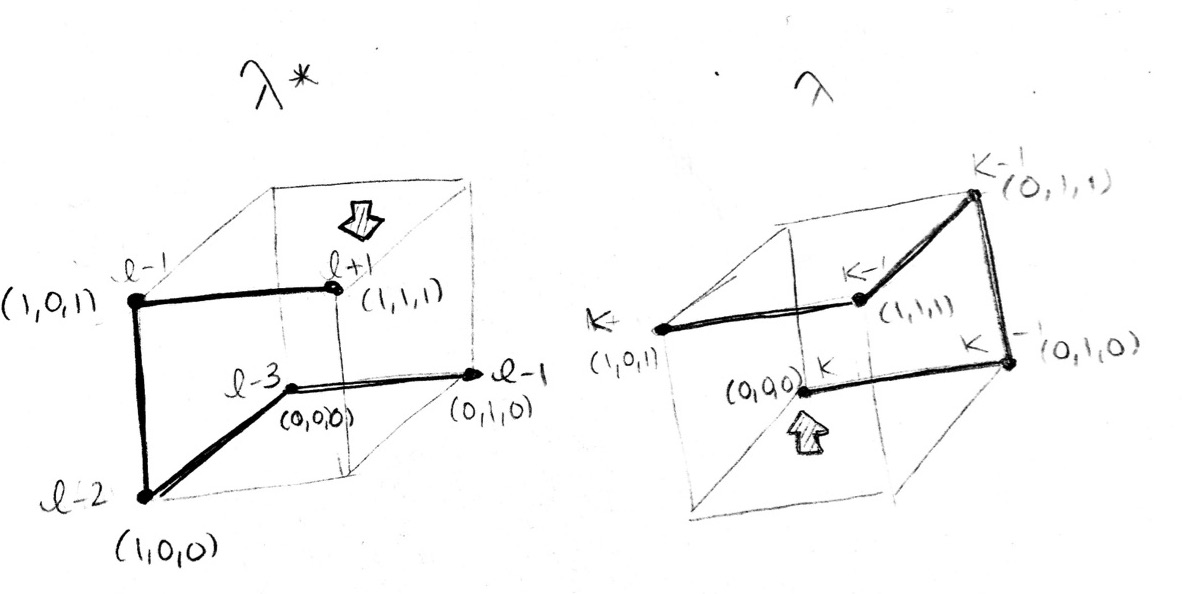
\includegraphics[scale=.4]{counterexample_d3.jpg}
\end{center}
This counterexample shows that $K$-$Pro$ and $PRo$ will not act in the same way on this tableau. It does not necessarily prove that the map is not equivariant, but it shows this proof method cannot be used. 
\end{document}